\documentclass[11pt, oneside]{article}   	% use "amsart" instead of "article" for AMSLaTeX format
\usepackage{geometry}                		% See geometry.pdf to learn the layout options. There are lots.
\geometry{letterpaper}                   		% ... or a4paper or a5paper or ... 
%\geometry{landscape}                		% Activate for for rotated page geometry
%\usepackage[parfill]{parskip}    		% Activate to begin paragraphs with an empty line rather than an indent
\usepackage{graphicx}				% Use pdf, png, jpg, or eps§ with pdflatex; use eps in DVI mode
								% TeX will automatically convert eps --> pdf in pdflatex		
\usepackage{amssymb}
\usepackage{amsmath}
\usepackage{parskip}
\usepackage{color}
\usepackage{hyperref}

\title{Integrating functions of a complex variable}
%\author{The Author}
%\section{}
%\subsection*{}
\date{}							% Activate to display a given date or no date

\graphicspath{{/Users/telliott_admin/Dropbox/Tex/png/}}
% \begin{center} 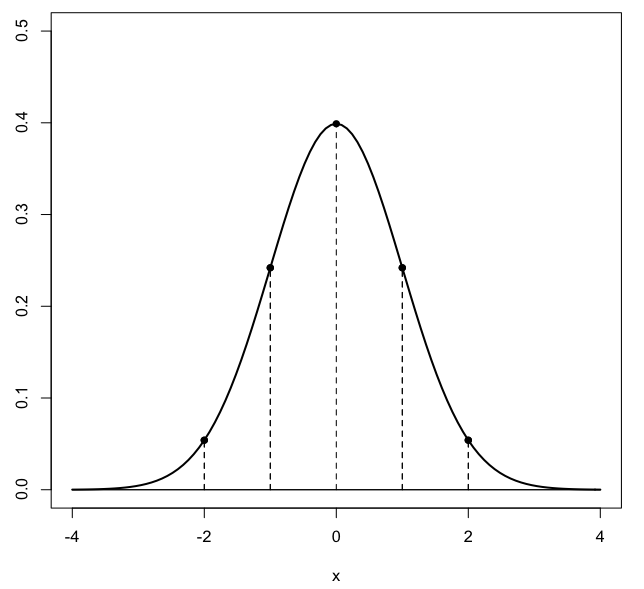
\includegraphics [scale=0.4] {gauss3.png} \end{center}
\begin{document}
\maketitle
\Large
If the contour (curve) of integration $C$ is parametrized in terms of $t$, then
\[ \int_C f(z) \ dz = \int_a^b f[z(t)] \ z'(t) \ dt \]

A particularly important parametrization is for circular paths.  On such a path, $z$ takes on values with constant $r$ and the only change is in $\theta$.  So we have
\[ z = re^{i \theta} \]
\[ z'(\theta) = i z \]
\[ dz = i z \ d \theta \]

As an example, consider $f(z) = z*$.

Note that this function is \emph{not} analytic, because it involves $z*$ rather than $z$, and secondly because
\[ z* = x - iy \]
so
\[ u_x = 1\ , \ \ \  v_y = - 1 \]
\[ u_x \ne v_y \]
The CRE do not hold.

Suppose our curve is the circle of radius $r$ centered at the origin, and we proceed between the endpoints $z = -ri \rightarrow ri$.  On this half-circle 
\[ z = re^{i \theta} \]
we have then
\[ dz = i \ re^{i \theta} \ d \theta \]
In radial coordinates
\[ z* = re^{-i\theta} \]
so we have
\[ \int {z*} \ dz = \int r e^{-i\theta} r i e^{i \theta} \ d \theta \]
\[ = r^2 i \int_{-\pi/2}^{\pi/2} d \theta = r^2 \pi i \]
Alternatively,
\[ zz* = |z|^2 = r^2  \]
\[ z* = \frac{r^2}{z} \]
\[ \int {z*} \ dz = r^2 \int \frac{1}{z} \ dz \]
Again
\[ z = re^{i \theta} \]
\[ dz = iz \ d \theta \]
So the integral is just
\[ = r^2 \int \frac{1}{z} \ iz \ d \theta   \]
\[ = r^2 i \int d \theta = r^2 \pi i \]

\subsection*{example}
Consider $f(z) = z^2$.  For the path, take the unit circle over the first quadrant from $(1,0)$ to $(0,1)$.  There is an easy way to do this, and a hard way.  Let's start by checking that this function is analytic, and then doing the hard way first.

Write $z$ in terms of $x$ and $y$:
\[ z = x + iy \]
\[ z^2 = (x + iy)^2 = x^2 - y^2 + i2xy \]
\[ u_x = 2x = v_y \]
\[ u_y = -2y = -v_x \]
The CRE hold.

Also
\[ dz = dx + i \ dy \]
So
\[ \int z^2 \ dz = \int (x^2 - y^2 + 2ixy) ( dx + i \ dy) \]
\[ = \int (x^2 - y^2) \ dx - \int 2 xy \ dy + i \int 2xy \ dx + i \int (x^2-y^2) \ dy \]
As before, we must parametrize this using the relationship between $x$ and $y$ along the curve.
\[ x = \cos t \]
\[ y = \sin t \]
\[ dx = - \sin t \ dt \]
\[ dy = \cos t \ dt \]
and then
\[ x^2 - y^2 = \cos^2 t - \sin^2 t = \cos 2t \]
\[ 2xy = 2 \cos t \sin t = \sin 2t \]
so the integral is
\[ = \int -\cos 2t \  \sin t \ dt - \int \sin 2t \ \cos t \ dt + \dots \]
\[ + \ i \ [ \ \int - \sin 2t \ \sin t \ dt + \int \cos 2t \ \cos t \ dt \]

Looks pretty wild!  In the book they use some trig identities I hadn't seen before, namely starting with the standard
\[ \sin s + t = \sin s \cos t + \sin t \cos s  \]
\[ \cos s + t = \cos s \cos t - \sin s \sin t \]
then, if $s = 2t$ then
\[ \sin 3t = \sin 2t \cos t + \sin t \cos 2t \]
\[ \cos 3t = \cos 2t \cos t - \sin 2t \sin t \]
Looking at the real part of the integral we had (combining terms)
\[ \int -\cos 2t \  \sin t - \sin 2t \ \cos t \ dt = \int - \sin 3t \ dt = \frac{\cos 3t}{3} \]
and for the imaginary part of the integral
\[ i \ [ \ \int - \sin 2t \ \sin t + \cos 2t \ \cos t \ dt = i \int \cos 3t \ dt = i \ \frac{\sin 3t}{3} \]
That looks a lot better.
\[ \frac{\cos 3t}{3} + i \ \frac{\sin 3t}{3} \ \bigg |_0^{\pi/2} = - \frac{1}{3} - i \ \frac{1}{3} = - \frac{1}{3} (1 + i) \]

For the easy way, just treat $z$ as if it were a real variable
\[ \int z^2 \ dz = \frac{z^3}{3} \ \bigg |_1^i = - \frac{1}{3} i - \frac{1}{3} \]
Note that if we go all the way around the unit circle the integral is just zero.

Going back to the first example we had
\[ \int z \ dz = \frac{z^2}{2} \ \bigg |_{1 + i}^{3 + 3i} \]
\[ = \frac{9 - 9 + 18i - \ [ \ 1 - 1 + 2i \ ] }{2} \]
\[ = 8i \]

\subsection*{example}
\[ \int_0^{2\pi} \frac{1}{z} \ dz \]

Examining the inverse function, let's first confirm that it is analytic by calculating the partial derivatives.  We have
\[ \frac{1}{z} = \frac{1}{x + iy} \]
Simplify by multiplying on top and bottom by $z*$:
\[ = \frac{1}{x + iy} \ \frac{x-iy}{x- iy} \]
\[ = \frac{x - iy}{x^2 + y^2} \]
Thus
\[ u = \frac{x}{x^2 + y^2} \]
\[ u_x = \frac{(x^2 + y^2) - 2x^2}{(x^2 + y^2)^2} = \frac{y^2 - x^2}{(x^2 + y^2)^2} \]
\[ u_y = \frac{-2xy}{(x^2 + y^2)^2} \]
And
\[ v =  \frac{-y}{x^2 + y^2} \]
\[ v_y = - \frac{(x^2 + y^2) - 2y^2}{(x^2 + y^2)^2} = \frac{y^2 - x^2}{(x^2 + y^2)^2} \]
\[ v_x = \frac{2xy}{(x^2 + y^2)^2} \]
CRE are satisfied and the inverse of $z$ is indeed analytic.

If we are on the unit circle, then 
\[ z = e^{i\theta} \]
\[ dz = ie^{i\theta} d \theta = iz\ d \theta \]
\[ \int \frac{dz}{z} = \int \frac{iz}{z} \ d \theta = 2 \pi i \]

If we're centered on the origin but we don't have a unit circle, there will be an $R$ in both the numerator and the denominator, which cancel.

The result is thus independent of the radius of the circle.

In general
\[ \oint_C \frac{dz}{(z - z_0)^n} = 
\begin{cases}
0, & n \ne 1 \\
2 \pi i, & n = 1 
\end {cases}
\]
(We will see examples for $n \ne 1$ below).

We can also integrate the inverse function in terms of $x$ and $y$:
\[ \oint \frac{1}{z} \ dz = \oint \frac{dx + i dy}{x + iy} \]
\[ = \oint \frac{1}{x^2+y^2} \ [ \  x \ dx - y \ dy + i x \ dy + i y \ dx \ ] \]
Suppose we go on a circle of radius $R$ centered on the origin and parametrize in terms of $\theta$.  We obtain:
\[ x = R \cos \theta \]
\[ y = R \sin \theta \]
\[ x^2 + y^2 = R^2 \]
\[ dx = - R \sin \theta \ d \theta \]
\[ dy = R \cos \theta \ d \theta \]
We have for the integral
\[ \oint \frac{1}{x^2+y^2} \ [ \  x \ dx - y \ dy + i x \ dy + i y \ dx \ ] \]
\[ = \int \frac{1}{R^2} \ [ \ -R^2 \cos \theta \sin \theta \ d \theta + R^2 \sin \theta \cos \theta \ d \theta + i R^2 \cos^2 \theta \ d \theta + i R^2 \sin^2 \theta \ d \theta \ ] \]
\[ = \int \frac{1}{R^2} \ [ \ i R^2 \cos^2 \theta \ d \theta + i R^2 \sin^2 \theta \ d \theta \ ] \]
\[ = \int \frac{1}{R^2} \ [ \ i R^2 \ d \theta \ ] \]
\[ = \int i \ d \theta = 2 \pi i \]

Note that if we integrate the same function around a unit square, we run into problems.  First let's  do $[0,0 \times 1,1]$.  We have
\[ \int u \ dx - \int v \ dy + i \ [ \ \int v \ dx + \int u \ dy \ ]  \]
Along $C1$, $y = 0$ and $dy = 0$ so:
\[ \int \frac{x}{x^2 + y^2} \ dx + i \ [ \ \int \frac{-y}{x^2 + y^2} \ dx \]
\[ = \int_0^1 \frac{1}{x} \ dx = \ln x \ \bigg |_0^1 \]
Since $\ln 0$ is not defined, we can't do this.

Logarithms are tricky, no doubt.  If the complex logarithm $Log z$ is defined and differentiable along the curve (say the semicircle from $-i$ to $i$), we can do this:
\[ I = \int_{-i}^i \frac{1}{z} \ dz = \text{ Log } z \ \bigg |_{-i}^i  \]
Recall that $z = re^{i\theta}$ with $r=1$ so this is
\[ = (\ln 1 + i \ \frac{\pi}{2} ) - (\ln 1 + i \frac{-\pi}{2} ) = 2i \ \frac{\pi}{2} = \pi i \]
For any value of $r$ (except $r=0$), we get the same answer, since $\ln r - \ln r = 0$.

\subsection*{example}
We can extend this to 
\[ \oint \frac{1}{z^2} \ dz \]
As before, on the unit circle
\[ z = e^{i\theta} \]
and
\[ \frac{dz}{d \theta} = i e^{i \theta} \]
so
\[ dz = i z \ d \theta \]
The integral is
\[ \int_0^{2 \pi} \ \frac{i}{z} \ d \theta =  i \int_0^{2 \pi} e^{-i\theta} \ d \theta \]
Now
\[ \int e^{-i\theta} \ d \theta = \frac{1}{-i} e^{-i\theta} = i e^{-i\theta} \]
so we have
\[ = - e^{-i\theta} \ \bigg |_0^{2 \pi}  \]
Evaluate at the upper bound using Euler's formula:
\[ e^{-2\pi i} = \cos -2 \pi + i \sin -2 \pi \]
\[ = \cos 2 \pi - i \sin 2 \pi = 1 \]
At the lower bound we also get $1$ so the whole thing is zero.

In fact, for any negative integer power of $z$
\[ \int z^{-n} \ dz \]
around the unit circle $z=e^{i\theta}$ we have
\[ i \int e^{-i(n-1)\theta} \ d \theta \]
\[ = -\frac{1}{n-1} \ e^{-i(n-1)\theta} \ \bigg |_0^{2 \pi}  \]
\[ = -\frac{1}{n-1} \ [ \ (\cos 2 (n-1) \pi - i \sin 2 (n-1) \pi ) \ - 1 ]   \]
\[ = -\frac{1}{n-1} \ [ \ 1  - 1 ] \ = 0  \]

\subsection*{example}
Consider
\[ \int \sqrt{z} \ dz \]
along the half-circle of radius $3$ starting from the point $z = R$ on the $x$-axis and proceeding counter-clockwise.
We can do this integral even if the "branch" of the square root function that we're using is only defined for $\theta > 0$.  We have that 
\[ z = Re^{i\theta}, \ \ \ \theta = 0 \rightarrow \pi \]
\[ dz = iz = iRe^{i\theta} \ d \theta \]
\[ \sqrt{z} = \sqrt{R} e^{i\theta/2} \]
so
\[ I = \int_0^{\pi} iR \sqrt{R} e^{i3\theta/2} \ d \theta \]
We need
\[ \int e^{i3\theta/2} \ d \theta = \frac{2}{3i} e^{i3\theta/2} \ \bigg |_0^{\pi} \]
easiest to write it out as
\[ e^{i3\theta/2} \ \bigg |_0^{\pi} = \cos \frac{3\pi}{2} + i \sin  \frac{3\pi}{2} - \cos 0 - i \sin 0 \]
\[ = 0 + i(-1) - 1 - 0 = -(1+i) \]
Going back to pick up all the factors we left behind:
\[ I = -iR \sqrt{R} \ \frac{2}{3i} \ (1+i) = -R \sqrt{R} \ \frac{2}{3} \ (1+i) \]
In the problem, $R$ was actually specified as $3$, leading to the cancellation:
\[ I = - 2 \sqrt{3} \ (1+i) \]

We can also do this problem by antiderivatives:
\[ \int_R^{-R} \sqrt{z} \ dz = \frac{2}{3} \ z^{3/2} \ \bigg |_R^{-R}  \]
\[ = \frac{2}{3} ( R^{3/2} e^{i3\pi/2} - R^{3/2} e^0) \]
\[ = \frac{2}{3} R^{3/2} ( e^{i3\pi/2} - 1) \]
and, as we showed above:
\[ e^{i3\pi/2} = -i \]
If $R=3$ we get the same answer as before.

\end{document}  